\chapter{Opis projektnog zadatka}
		
		Cilj ovog projekta je izrada mobilne aplikacije „Inventura“ koja će korisniku olakšati posao inventure skladišta. Tvrtke čiji zaposlenici će koristiti ovu aplikaciju imaju nekoliko skladišta na različitim lokacijama te će pomoću ove aplikacije i mobilne kamare moći očitati bar kodove i QR kodove artikala čiju inventuru žele napraviti. Također, ovisno o tome koju ulogu u tvrtci korisnik ima, aplikacija mu nudi određene funkcionalnosti kao što su: prikaz informacija o artiklu, njegova lokacija, broj artikala, mogućnost povećanja i smanjenja broja artikala, spremanje promjena u bazu, slanje obavijesti nadležnima, kontrola inventure, preraspodjela artikala po grupama i mnoge druge.
		
		Prilikom pokretanja aplikacije korisniku se prikazuje stranica za prijavu registriranih korisnika na kojoj se nalaze polja za unos email adrese i lozinke. Neregistrirani korisnik pri dnu stranice za prijavu treba odabrati opciju „Registriraj se“ koja ga vodi na stranicu za registraciju. Za kreiranje novog računa potrebno je navesti:
		
		\begin{packed_item}
			\item \textit{Ime}
			\item \textit{Prezime}
			\item \textit{Email}
			\item \textit{Lozinku}
			\item \textit{Ulogu u tvrtci}
			\item \textit{Ovisno o ulozi u tvrtci, skladište u kojem zaposlenik radi}
		\end{packed_item}
	
		Kada se korisnik prijavi u sustav uključuje mu se stražnja kamera mobilnog uređaja te se prikazuje početni zaslon koji je spreman za očitavanje bar koda i QR koda. Osim što može očitati kodove, korisnik ovisno o svojoj ulozi ima još dodatnih mogućnosti.
		
		\underbar{Korisnik može imati jednu od ove tri uloge:}
		\begin{packed_item}
			\item \textit{Skladištar}
			\item \textit{Šef skladišta}
			\item \textit{Direktor}
		\end{packed_item}
	
		\underbar{Skladištar} je osoba koja obavlja inventuru skladišta te po potrebi obavještava svoje nadležne ako određenog artikla nema na skladištu. Biranje artikla za skeniranje se vrši automatski, na način da prvi artikl koji skenira u toj inventuri je onaj odabrani. Zatim se uključi stražnja kamera mobilnog uređaja te se na ekranu aplikacije prikazuje početni zaslon koji je spreman za skeniranje. Kada se na proizvodu skenira te mu se detektira bar kod ili QR kod, skladištaru na zaslonu aplikacije iskače prozor (engl.\emph{pop-up window}) koji se prikazuje 5 sekundi. Taj prozor sadrži informacije o skeniranom proizvodu u obliku kratkog opisa, lokaciju na kojoj je skeniran (dohvaćenu automatski pomoću GPS modula mobitela) i brojač takvih proizvoda u skladištu, a također i nudi opcije povećanja i smanjenja broja proizvoda, odbacivanje trenutnog očitanja bez spremanja u bazu, te pohranu trenutnog očitanja u bazu bez čekanja da istekne 5 sekundi. Promjenom broja očitanih artikala resetira se brojač 5 sekundi, a istekom vremena brojača zapis se automatski sprema u bazu. Na početnom zaslonu postoji i opcija \emph{Završi}. Odabirom te opcije skladištar završava svoj rad nad tim proizvodom. Svaki skladištar može skenirati samo jednu vrstu proizvoda dok ne označi završetak skeniranja tog proizvoda. Osim opcije za skeniranje proizvoda, skladištaru se na početnoj stranici nudi još i mogućnost odjave iz aplikacije te povijest svih unosa proizvoda. Odabirom prikaza povijesti, sustav korisniku prikazuje pregled povijesti svih unosa korisnika. Prvo prema odrađenim inventurama, uz koje se prikazuje datum inventure. Pritiskom na izabranu inventuru prikazuju se svi proizvodi koje je prijavljeni skladištar unio u aplikaciju, dok pritiskom na još aktivnu inventuru, uza sve unesene proizvode skladištar može dojaviti šefu skladišta da nekog artikla nema na skladištu. Prilikom pregleda povijesti unosa, za svaki artikl navodi se njegov naziv, lokacija na kojoj je skeniran te broj koliko je takvih artikala prijavljeni skladištar skenirao.
		
		\underbar{Šef skladišta}, za razliku od ostalih korisnika, ima mogućnost korištenja aplikacije na 1 od 2 načina: kao izvršitelj inventure ili kao kontrolor inventure. Prilikom ulaska u aplikaciju otvara mu se kamera za detekciju bar kodova i QR kodova. Ukoliko je skenirao proizvod koji u trenutnoj inventuri nije bio skeniran tada ima ulogu izvršitelja inventure. Za razliku od toga, ako je proizvod već skeniran u trenutnoj inventuri, tada ima ulogu kontrolora inventure.\\Kao izvršitelj inventure, dobiva jednaku funkcionalnost kao i skladištar i uključuje mu se kamera mobilnog uređaja. Zatim se na ekranu aplikacije prikazuje početni zaslon koji je spreman za skeniranje. Kada se proizvodu skenira i detektira bar kod ili QR kod, šefu skladišta na zaslonu aplikacije iskače prozor (engl. \emph{pop-up window}) koji se prikazuje 5 sekundi. Taj prozor sadrži informacije o skeniranom proizvodu, lokaciju na kojoj je skeniran (automatsko dohvaćanje pomoću GPS modula mobitela) i brojač takvih proizvoda u skladištu te nudi opcije povećanja i smanjenja broja proizvoda, odbacivanje trenutnog očitanja bez spremanja u bazu te pohranu trenutnog očitanja u bazu bez čekanja da istekne 5 sekundi. Promjenom broja očitanih artikala resetira se brojač 5 sekundi, a istekom vremena brojača zapis se automatski sprema u bazu. Na početnom zaslonu postoji i opcija \emph{Završi}. Odabirom te opcije označava se završetak skeniranja odabranog artikla. Osim opcije za skeniranje proizvoda, šefu skladišta se nude još četiri mogućosti na početnom zaslonu: pregled svih artikala na skladištu, pregled svih izvršenih inventura nad tim skladištem, pregled obavijesti te izlazak (odjava) iz aplikacije. Odabirom prikaza povijest prikazuje se pregled povijesti svih unosa korisnika. Prvo prema odrađenim inventurama, uz koje se prikazuje datum inventure. Odabirom određene inventure, šefu skladišta se nudi opcija pregleda svih artikala na skladištu tako da se za svaki artikl ispisuje njegov naziv, lokacija te broj takvih artikala na skladištu. Odabirom prikaza pošte na početnom zaslonu, šefu skladišta se otvara stranica s obavijestima. Navedene obavijesti poslali su skladištari koji su uočili da određenih artikala nema na skladištu. Odabirom opcije prikaza svih proizvoda, šef skladišta može vidjeti sve artikle koji se trenutno nalaze na njegovom skladištu.\\Kao kontrolor inventure šef skladišta ima iste funkcionalnosti kao i skladištari. Jedina razlika je što odabirom opcije \emph{Završi}, ukoliko je broj skeniranih artikala od strane šefa skladišta različit od broja koje je skenirao skladištar, aplikacija automatski o tome obavještava direktora.
		
		\underbar{Direktor tvrtke} je korisnik aplikacije kojem su omogućene najveće funkcionalnosti i koji ima pristup gotovo svim do sad navedenim mogućnostima. Naime, nakon prijave u sustav otvara mu se početni zaslon i uključuje stražnja kamera mobilnog uređaja kako bi mogao skenirati artikl. Kada se proizvodu skenira i detektira bar kod ili QR kod, direktoru na zaslonu aplikacije iskače prozor (engl. \emph{pop-up window}) koji se prikazuje 5 sekundi. Taj prozor sadrži informacije o skeniranom proizvodu, lokaciju na kojoj je skeniran (automatsko dohvaćanje pomoću GPS modula mobitela) i brojač takvih proizvoda u skladištu te nudi opcije povećanja i smanjenja broja proizvoda, odbacivanje trenutnog očitanja bez spremanja u bazu te pohranu trenutnog očitanja u bazu bez čekanja da istekne 5 sekundi. Promjenom broja očitanih artikala resetira se brojač 5 sekundi, a istekom vremena brojača zapis se automatski sprema u bazu. Na zaslonu postoji i opcija \emph{Završi sken} čijim se odabirom završava rad nad tim artiklom, kao i opcija \emph{Završi inventuru} čijim se odabirom završava trenutna inventura te automatski počinje nova. Osim opcije za skeniranje proizvoda, direktoru tvrtke nude se još tri mogućnosti na početnom zaslonu: pregled svih skladišta u kojima se obavljala inventura, pregled obavijesti te izlazak (odjava) iz aplikacije. Odabirom svih inventura direktoru se nudi opcija pregleda svih skladišta u kojima se obavljala inventura. Nakon što direktor odabere određeno skladište, otvara mu se nova stranica na kojoj može odabrati želi li pretraživati skladištare koji su obavljali inventure ili artikle koji su bili skenirani. Ako odabere opciju \emph{Artikli} prikazuju mu se svi skenirani artikli u tom skladištu, te za svaki artikl njegovo ime i broj takvih artikala u odabranom skladištu. Osim što ima uvid u postojeće artikle, odabirom dodavanja novih kategorija direktoru se nudi opcija dodavanja grupa proizvoda i preraspodjela artikala po grupama. Za te funkcionalnosti otvara mu se nova stranica u kojoj može dodati novu grupu proizvoda, otići na već postojeću grupu ili preraspodijeliti artikle po grupama. Grupe proizvoda su organizirane u stablo s korijenom „proizvod“, a dubina i širina stabla nisu ograničeni. Osim opcije \emph{Artikli} postoji i opcija \emph{Skladištari} koja direktoru tvrtke prikazuje ime skladištara koji je radio inventuru u odabranom skladištu te njegovu statistiku pogreške. Odabirom popisa skladišta, prikazuje se ponovno popis svih skladišta, ali pritiskom na jedno od skladišta otvara se nova stranica s popisom svih inventura na tom skladištu. Odabirom određene inventure, direktor ima uvid u sve proizvode koji su se skenirali u toj inventuri. Odabirom opcije pregleda obavijesti, direktoru tvrtke otvara se stranica s obavijestima koje su poslali šefovi skladišta. Navedene obavijesti direktor može označiti odabirom odgovarajuće opcije kao riješene ili kao odbačene. Također, direktor ima pristup povijesti svih obavijesti.\\
		
		\large{\textbf{\textit{Postojeća slična rješenja}}}\normalsize
		
		\underbar{\textbf{1. EZOfficeInventory}}
		
		Jedna od popularnih aplikacija za vođenje inventure je EZOfficeInventory, aplikacija koja na bazi QR koda i bar koda omogućava skeniranje i praćenje inventure. Uz samo skeniranje kodova pomoću aplikacije, omogućuje povezivanje i RIFD čitača za olakšanu primjenu. Kako bi se lakše pratili proizvodi unutar skladišta omogućeno je i praćenje statistike podjeljive na više lokacija, timova itd., te podjelu ljudi po ulogama unutar same firme.
		
		\begin{figure}[H]
			
\includegraphics[height=5cm]{slike/EZ_logo.png}
			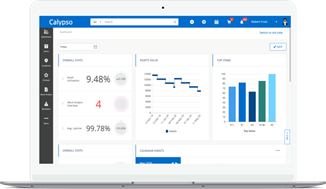
\includegraphics[height=5cm]{slike/EZ_slika.png}
			\centering
			\label{ez_logo}
		\end{figure}
		
		\underbar{\textbf{2. CountIt - Inventory application}}
		
		CountIt omogućava povezivanje više mobilnih uređaja na više lokacija skladišta te sve promjene sprema na oblak. Praćenje broja uživo, skeniranje podataka i spremanje uživo na oblak. Uz to, aplikacija omogućuje i dodjelu poslova, statistike praćenja cijele inventure te prilično fleksibilan plan korištenja, jeftiniji od ostalih konkurenata te se može bilo kada otkazati (za veće grupe i više opcija skuplje).
		
		\begin{figure}[H]
			
\includegraphics[height=5cm]{slike/CT_logo.png}
			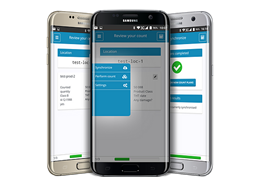
\includegraphics[height=5cm]{slike/CT_slika.png}
			\centering
			\label{ct_logo}
		\end{figure}
		
		\underbar{\textbf{3. Erply: Stocktake app}}
		
		Erply, uz dosadašnje implementacije različitih funkcija, nudi i offline brojanje artikla (prilikom spremanja u bazu naravno ponovno mora ići online ili prebaciti podatke na računalo kablom), pomoću povijesti skeniranih kodova nudi brže prepoznavanje i samo skeniranje, notifikacije korisnicima ukoliko se broj proizvoda previše smanji.
		
		\begin{figure}[H]
			
\includegraphics[height=5cm]{slike/ER_logo.png}
			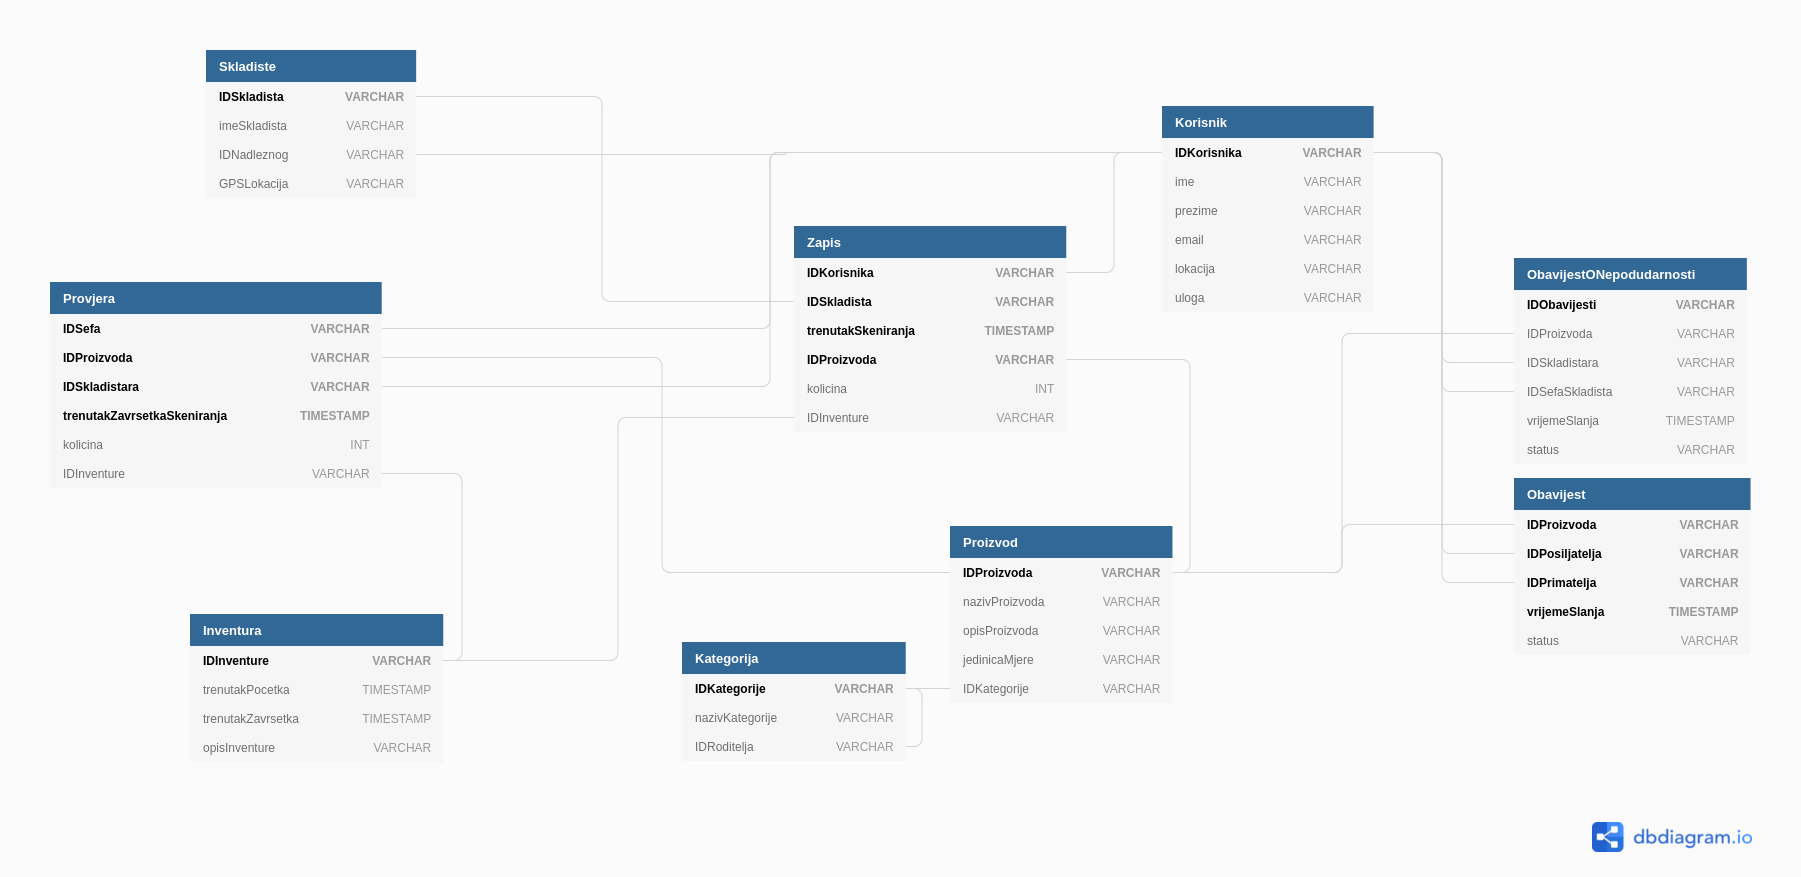
\includegraphics[height=5cm]{slike/ER_slika.png}
			\centering
			\label{er_logo}
		\end{figure}
		
		\underbar{\textbf{4. Stockpile by Canvus}}
		
		Besplatna i jednostavnija verzija dosadašnjih aplikacija koja se fokusira na manje privatne firme kako bi im olakšali provođenje inventure. Aplikacija, za razliku od ostalih, ne nudi skeniranje kodova proizvoda, ali sadrži osnovne funkcionalnosti potrebne za provođenje inventure.
		
		\begin{figure}[H]
			
\includegraphics[width=0.49\linewidth]{slike/ST_logo.png}
			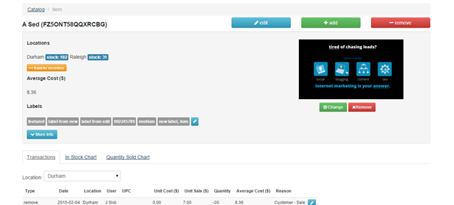
\includegraphics[width=0.49\linewidth]{slike/ST_slika.png}
			\centering
			\label{st_logo}
		\end{figure}
		
		\bigskip
				
		\large\textbf{\textit{Tržište i ciljana skupina}}\normalsize
		
		Ciljana skupina su tvrtke koje posjeduju veliki broj skladišta na brojnim i udaljenim lokacijama te im je tako proces inventure otežan. Tržište su sve kompanije koje posjeduju skladišta, posebice kompanije koje rade kontinuirane inventure.\\
		
		\large\textbf{\textit{Opseg projektnog zadatka}}\normalsize
		
		Aplikacija se sastoji od intuitivnog korisničkog sučelja, a osnovne su funkcionalnosti detekcija i skeniranje QR ili bar kodova artikala u skladištu prilikom inventure. Svaki korisnik mora moći skenirati artikle, a ostale funkcionalnosti se dijele prema razini pristupa. Direktor ima pristup svim funkcionalnostima aplikacije, između ostaloga uvid u sva skladišta, artikle i statistiku pogrešaka pojedinog skladištara. Važna funkcionalnost je dodavanje artikala u stablo proizvoda. Pristup toj funkcionalnosti ima samo direktor tvrtke. Također, aplikacija mora omogućiti svakom skladištaru skeniranje samo jedne vrste artikala dok ne završi s prebrojavanjem te vrste artikla. Svaki korisnik može se prijaviti, registrirati ako nema napravljen račun, kao i odjaviti ako želi.\\
		
		\large\textbf{\textit{Moguće nadogradnje projektnog zadatka}}\normalsize
		
		Projektni zadatak mogao bi se nadograditi integracijom s nekom od popularnih aplikacija za upravljanje timom (npr. \emph{Slack}). Tako bismo ubacili opciju međusobne komunikacije između članova tvrtke. Osim automatski generiranih poruka koje aplikacija nudi, svi članovi kompanije mogli bi razmjenjivati poruke međusobno. Uz to, jedna od mogućih nadogradnji svakako je višejezičnost. Aplikacija bi mogla evidentirati nabavne i prodajne naloge te automatski dodavati odnosno oduzimati broj artikala ovisno o njihovoj prodaji ili nabavi.\\
		
		
		Za pomoć pogledati reference navedene u poglavlju „Popis literature“, a po potrebi konzultirati sadržaj na internetu koji nudi dobre smjernice u tom pogledu.
		\eject
		
		\begin{comment}
		\section{Primjeri u \LaTeX u}
		
		\textit{Ovo potpoglavlje izbrisati.}\\

		U nastavku se nalaze različiti primjeri kako koristiti osnovne funkcionalnosti \LaTeX a koje su potrebne za izradu dokumentacije. Za dodatnu pomoć obratiti se asistentu na projektu ili potražiti upute na sljedećim web sjedištima:
		\begin{itemize}
			\item Upute za izradu diplomskog rada u \LaTeX u - \url{https://www.fer.unizg.hr/_download/repository/LaTeX-upute.pdf}
			\item \LaTeX\ projekt - \url{https://www.latex-project.org/help/}
			\item StackExchange za Tex - \url{https://tex.stackexchange.com/}\\
		
		\end{itemize} 	


		
		\noindent \underbar{podcrtani tekst}, \textbf{podebljani tekst}, 	\textit{nagnuti tekst}\\
		\noindent \normalsize primjer \large primjer \Large primjer \LARGE {primjer} \huge {primjer} \Huge primjer \normalsize
				
		\begin{packed_item}
			
			\item  primjer
			\item  primjer
			\item  primjer
			\item[] \begin{packed_enum}
				\item primjer
				\item[] \begin{packed_enum}
					\item[1.a] primjer
					\item[b] primjer
				\end{packed_enum}
				\item primjer
			\end{packed_enum}
			
		\end{packed_item}
		
		\noindent primjer url-a: \url{https://www.fer.unizg.hr/predmet/proinz/projekt}
		
		\noindent posebni znakovi: \# \$ \% \& \{ \} \_ 
		$|$ $<$ $>$ 
		\^{} 
		\~{} 
		$\backslash$ 
		
		
		\begin{longtblr}[
			label=none,
			entry=none
			]{
				width = \textwidth,
				colspec={|X[8,l]|X[8, l]|X[16, l]|}, 
				rowhead = 1,
			} %definicija širine tablice, širine stupaca, poravnanje i broja redaka naslova tablice
			\hline \multicolumn{3}{|c|}{\textbf{naslov unutar tablice}}	 \\ \hline[3pt]
			\SetCell{LightGreen}IDKorisnik & INT	&  	Lorem ipsum dolor sit amet, consectetur adipiscing elit, sed do eiusmod  	\\ \hline
			korisnickoIme	& VARCHAR &   	\\ \hline 
			email & VARCHAR &   \\ \hline 
			ime & VARCHAR	&  		\\ \hline 
			\SetCell{LightBlue} primjer	& VARCHAR &   	\\ \hline 
		\end{longtblr}
		

		\begin{longtblr}[
				caption = {Naslov s referencom izvan tablice},
				entry = {Short Caption},
			]{
				width = \textwidth, 
				colspec = {|X[8,l]|X[8,l]|X[16,l]|}, 
				rowhead = 1,
			}
			\hline
			\SetCell{LightGreen}IDKorisnik & INT	&  	Lorem ipsum dolor sit amet, consectetur adipiscing elit, sed do eiusmod  	\\ \hline
			korisnickoIme	& VARCHAR &   	\\ \hline 
			email & VARCHAR &   \\ \hline 
			ime & VARCHAR	&  		\\ \hline 
			\SetCell{LightBlue} primjer	& VARCHAR &   	\\ \hline 
		\end{longtblr}
	


		
		
		%unos slike
		\begin{figure}[H]
			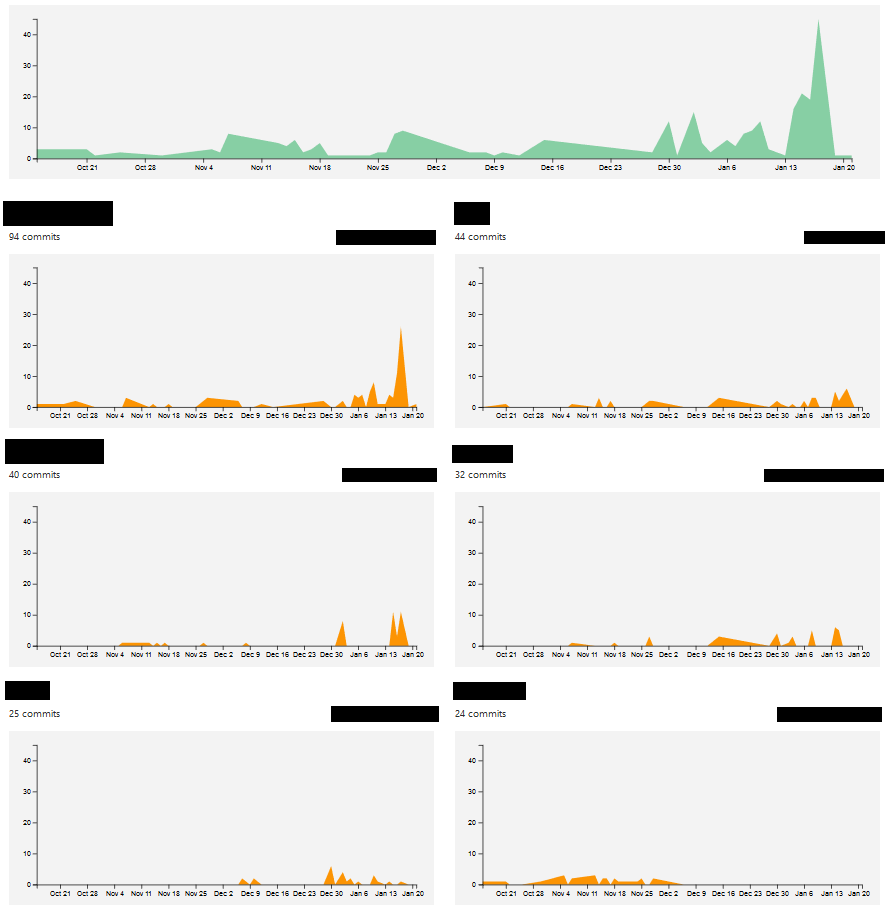
\includegraphics[scale=0.4]{slike/aktivnost.png} %veličina slike u odnosu na originalnu datoteku i pozicija slike
			\centering
			\caption{Primjer slike s potpisom}
			\label{fig:promjene}
		\end{figure}
		
		\begin{figure}[H]
			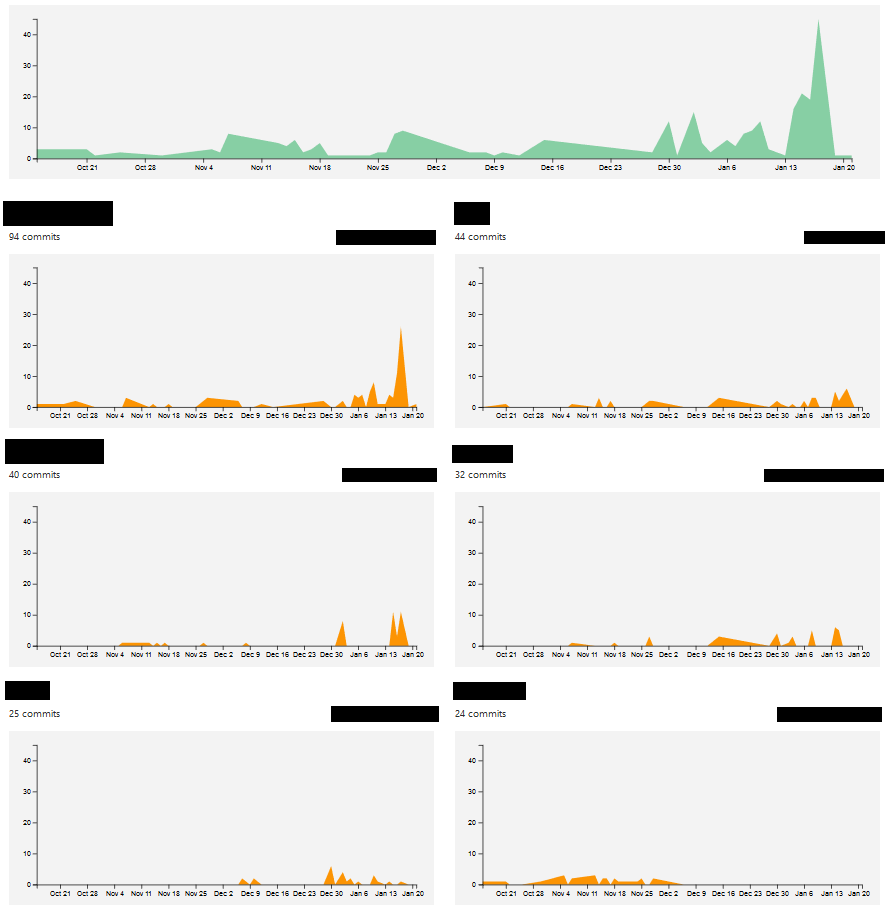
\includegraphics[width=\textwidth]{slike/aktivnost.png} %veličina u odnosu na širinu linije
			\caption{Primjer slike s potpisom 2}
			\label{fig:promjene2} %label mora biti drugaciji za svaku sliku
		\end{figure}
		
		Referenciranje slike \ref{fig:promjene2} u tekstu.
		
		\eject
		\end{comment}
		
	